\documentclass[hidelinks,11pt,dvipsnames]{article}
% xcolor commonly causes option clashes, this fixes that
\PassOptionsToPackage{dvipsnames,table}{xcolor}
\usepackage[tmargin=1in, bmargin=1in, lmargin=0.8in, rmargin=1in]{geometry}

%%%%%%%%%%%%%%%%%%%%%%%%%%%%%%%%%%%%%%%%%%%%%%%%%%%%%%%%%%%%%%%%%%%%
%%% For inkscape-figures
%%% Assumes the following directory structure:
%%% master.tex
%%% figures/
%%%     figure1.pdf_tex
%%%     figure1.svg
%%%     figure1.pdf
%%%%%%%%%%%%%%%%%%%%%%%%%%%%%%%%%%%%%%%%%%%%%%%%%%%%%%%%%%%%%%%%%%%%
%\usepackage{import}
\usepackage{pdfpages}
\usepackage{transparent}

\newcommand{\incfig}[2][1]{%
    \def\svgwidth{#1\columnwidth}
    \import{./figures/}{#2.pdf_tex}
}

\pdfsuppresswarningpagegroup=1

% enable synctex for inverse search, whatever synctex is
\synctex=1
\usepackage{float,macrosabound,homework,theorem-env}
\usepackage{microtype}


% font stuff
\usepackage{sectsty}
\allsectionsfont{\sffamily}
\linespread{1.1}

% bibtex stuff
\usepackage[backend=biber,style=alphabetic,sorting=anyt]{biblatex}
\addbibresource{main.bib}

% colored text shortcuts
\newcommand{\blue}[1]{\color{MidnightBlue}{#1}}
\newcommand{\red}[1]{\textcolor{Mahogany}{#1}}
\newcommand{\green}[1]{\textcolor{ForestGreen}{#1}}


% use mathptmx pkg while using default mathcal font
\DeclareMathAlphabet{\mathcal}{OMS}{cmsy}{m}{n}

% fixes the positioning of subscripts in $$ $$
\renewcommand{\det}{\operatorname{det}}

\usetikzlibrary{positioning, arrows.meta}
\newcommand{\here}[2]{\tikz[remember picture]{\node[inner sep=0](#2){#1}}}

%%%%%%%%%%%%%%%%%%%%%%%%%%%%%%%%%%%%%%%%%%%%%%%%%%%%%%%%%%%%%%%%%%%%%
%%% Entry Counter
%%%%%%%%%%%%%%%%%%%%%%%%%%%%%%%%%%%%%%%%%%%%%%%%%%%%%%%%%%%%%%%%%%%%%
\newcounter{entry-counter}
\newcommand{\entry}[1]
{
	\addtocounter{entry-counter}{1}
    \tchap{Entry \arabic{entry-counter}}
	%\addcontentsline{toc}{section}{Entry \arabic{entry-counter}: #1}
	\vspace{-1.5em}
    \begin{center}
		\small \emph{Written: #1}
    \end{center}
}

\usepackage{titling}
\renewcommand\maketitlehooka{\null\mbox{}\vfill}
\renewcommand\maketitlehookd{\vfill\null}


\def\sset{\subseteq}
\def\iso{\cong}
\def\gend#1{\langle #1\rangle}

\begin{document}
\pagestyle{empty}
	\LARGE
\begin{center}
	Algebraic Topology Homework 0 \\
	\Large
	Isaac Martin \\
    Last compiled \today
\end{center}
\normalsize
\vspace{-2mm}
\hru
\begin{homework}[e]
    \prob Suppose you take the disjoint union of finitely many triangles, and identify their edges in pairs, by some affine homeomorphisms.  Prove that the result is a manifold.

    (Following Hatcher, an $n$-dimensional manifold means a Hausdorff topological space, each of whose points has an open neighborhood that is homeomorphic to $\bR^n$. Many other sources include the extra technical hypothesis of \emph{paracompactness}.)
	\begin{prf}
		Let $T_1,...,T_n \subseteq \bR^2$ denote the triangles in question. It will not be important to distinguish between the three edges of an individual triangle all the edges and gluing maps of these triangles explicitly, instead, we will refer to \emph{an} edge $e_{ij}$ of triangle $T_i$ glued to \emph{an} edge $e_{ji}$ of triangle $T_j$ via a gluing homeomorphism $\varphi_{ij}:e_{ij}\to e_{ji}$. Let $X = \coprod_{i = 1}^n T_i /\sim$ where $x \sim y$ if $x \in e_{ij}$ and $y \in e_{ji}$ for some $i,j$ such that $\varphi_{ij}(x) = y$. The topology on each $T_i$ is the subspace topology and the topology on $X$ is the quotient topology. Finally, let $\pi:\coprod_{i = 1}^n T_i \to X$ denote the projection map.

		We first show that $X$ is Hausdorff. Choose two distinct points $x,y \in X$. Pulling back into $\coprod_{i=1}^n T_i$, we may find separating open neighborhoods $U$ for $x$ and $V$ for $y$ in $\coprod_{i=1}^n T_i$, since each $T_i$ inherits Hausdorffness from $\bR^2$. Up to relabeling, we may assume $T_1,...,T_k$ are the triangles containing $\pi^{-1}(\{x,y\})$. These are all open in the disjoint union topology, so by intersecting with $U$ and $V$ and pushing forward to $X$, we obtain open separating neighborhoods for $x$ and $y$ in $X$.

		Our task is now to show that for any point $x \in X$ we can find an open neighborhood $U \subseteq X$ which is homeomorphic to $\bR^2$. It suffices to show that we can find such a neighborhood which is homeomorphic to an open disk in $\bR^2$. If $x$ is contained in the interior of a triangle $T_i$, then we may find an open ball $B \subseteq T_i$ containing $x$ which is entirely contained in the interior. As no gluing occurs on the interiors of the triangle, $\pi|_B$ is a homeomorphism onto its image. As $B$ is an open ball in the interior $T_i^{\text{int}}$ of $T_i$, $B = B' \cap T^{\text{int}}_i = B'$ for some open ball $B'$ in $\bR^2$. Thus, $\pi|_B$ is a homeomorphism from a neighborhood of $x$ to an open ball in $X$, as desired.

		Suppose instead that $x \in X$ occurs on an edge of one of the triangles. We treat both the case that $x$ is a vertex and the case that $x$ is not a vertex simultaneously. By relabeling the triangles if necessary, we may assume $\pi^{-1}(x) \subseteq T_1\cup...\cup T_k$. Let $U$ denote the interior of $\pi(T_1\cap ...\cap T_k)$, and note that this is an open neighborhood of $x$ in $X$. We show that $U$ is homeomorphic to an open ball in $\bR^2$.

		Set $U_i = \pi^{-1}(U) \cap T_i$. Each $U_i$ looks like a triangle with all edges avoiding $\pi^{-1}(x)$ removed. Both $\pi^{-1}(U)$ and $T_i$ are open in $\coprod_{i=1}^n T_i$, the former due to the continuity of $\pi$ and the latter due to the definition of the disjoint union topology, hence $U_i$ is open in $T_i$ and can be realized as the intersection of $T_i$ with an open set $A_i \subseteq \bR^2$. In fact, as $U_i$ is simply connected, we may assume $A_i$ is simply connected in $\bR^2$. All open simply connected sets in $\bR^2$ are homeomorphic to the open unit ball $B$ (c.f. the Riemann mapping theorem), so we have homeomorphism $\psi_i:A_i \to B$ for each $1\leq i\leq k$.

		This is the most hand-wavy portion of the argument. I claim without proof that we can choose the $\psi_i$ in such a way that whenever $\varphi_{ij}(a) = b$, we have that $\psi_i(a) = \psi_j(b)$ in $B$. By deforming the image of $\psi_i$ by homeomorphisms if necessary, we may further assume that $\psi_i(U_i) \cap \psi_j(U_j) = \psi_i(e_{ij} \cap U_i) = \psi_j(e_{ji} \cap U_j)$, i.e. That the images of the $U_i$ in $B$ under their $\psi_i$ maps meet only along adjacent edges. 

		For a point $y \in U$, we have at most one point $y_i \in U_i$ such that $\pi(y_i) = y$. Hence, we can define a map $f:U \to B$ by
		\begin{align*}
			f(y) = \psi_i(y_i) \text{ where $i$ is chosen such that } \pi^{-1}(y)\cap U_i = \{y_i\}.
		\end{align*}
		In the event that there are multiple valid choices for $i$, our assumption that $\psi_i$ and $\psi_j$ agree on edges wherever they are defined ensures $f$ is still well defined. To show $f$ is a homeomorphism, I provide a picture. See figure (\ref{fig:prob1}).
	\end{prf}

	\begin{figure}[h]
		\centering
		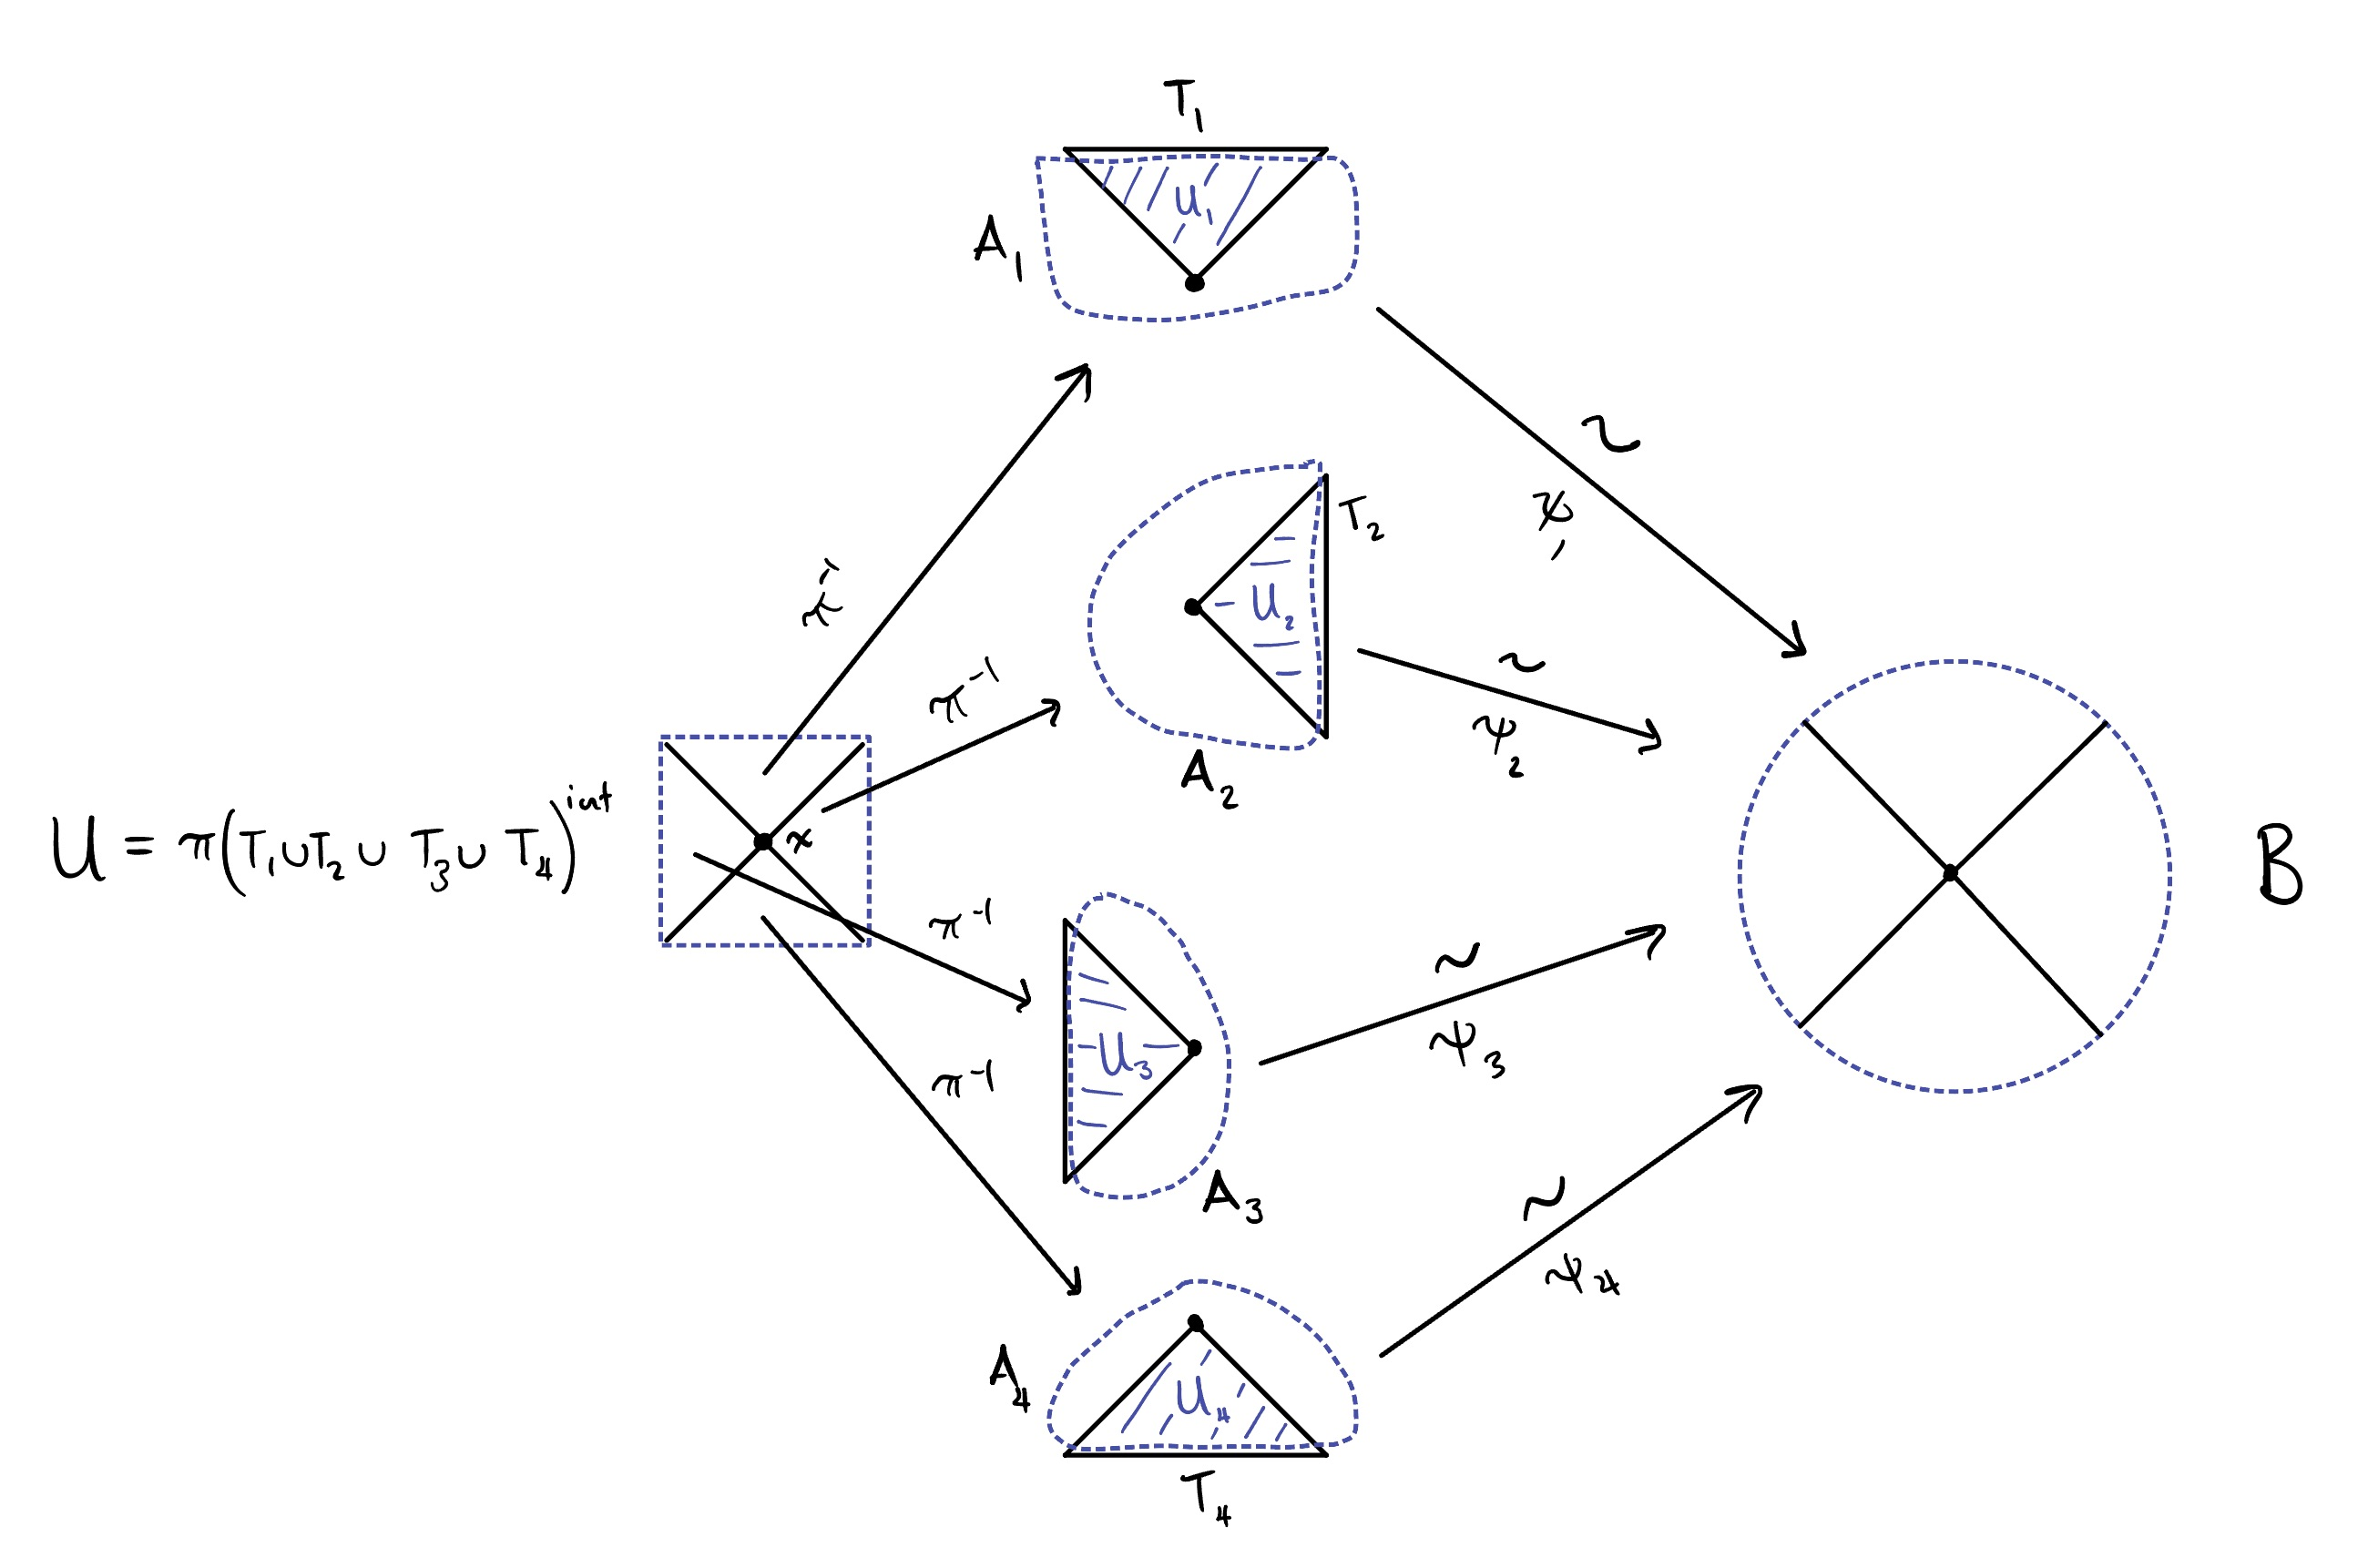
\includegraphics[width=15cm]{./figures/hwk0-fig.png}
		\caption{Accompanying figure attempting to elucidate the thought process in Problem 1.}
		\label{fig:prob1}
	\end{figure}

	\prob Suppose a finite group $G$ acts on a manifold~$M$.  Suppose the action is \emph{free}, meaning that only the identity element has any fixed points.  Then the orbit space $M/G$ is also a manifold.  (``Lying in the same $G$-orbit'' is an equivalence relation on~$M$.  $M/G$ means the set of equivalence classes.  The topology on $M$ induces one on $M/G$, which is the one you must work with.)
	\begin{prf}
		Let $M$ be an $n$-manifold and let $\pi:M\to M/G$ be the projection map. We prove that $M/G$ is an $n$-manifold in three parts:
		\begin{enumerate}[(1)]
			\item we show $\pi:M\to M/G$ is an open map,
			\item we show $M/G$ is Hausdorff and 
			\item for an arbitrary $x \in M/G$ we find an open neighborhood $U$ of $x$ such that $U \cong \bR^n$.
		\end{enumerate}
		\noindent (1): \hspace{1em} We first establish that $\pi$ is open. Indeed, if $U \subseteq M$ is an open set, then I claim
		\begin{align*}
			\pi^{-1}(\pi(U)) = \bigcup_{g\in G} g(U).
		\end{align*}
		Each $g$ acts by homeomorphism on $M$, and hence $\pi^{-1}(\pi(U))$ is itself open as it is a union of open sets. 

		If $x \in \pi^{-1}(\pi(U))$ then $\pi(x) \in \pi(U)$, so there is some $g,h \in G$ such that $gx \in h(U) \implies x \in g^{-1}h(U)$. This gives the forward inclusion.

		If $x \in g(U)$ for some $g \in G$, then $g^{-1}x \in U \implies \pi(x) = \pi(g^{-1}x) \in \pi(U)$. This means $x \in \pi^{-1}(\pi(U))$, and we have our result.

		\bigskip

		\noindent (2): \hspace{1em} We now argue that $M/G$ is Hausdorff. Consider two cosets $\olx,\oly \in M/G$ and let $x$ and $y$ be representatives for $\olx$ and $\oly$ respectively. Since $M$ is Hausdorff and $\oly \subseteq M$ is finite, we may find an open neighborhood $U$ of $x$ such that $U \cap \oly = \emptyset$. Similarly, we may find an open neighborhood $V$ of $y$ such that $V \cap \oly = \emptyset$. Then $\pi(U)$ and $\pi(V)$ are open neighborhoods of $\olx$ and $\oly$ respectively by part (1) and have trivial intersection since $U \cap \oly = V \cap \oly = \emptyset$. Hence, $M/G$ is Hausdorff.

		\bigskip

		\noindent (3): \hspace{1em} Fix $\olx \in M/G$ and a representative $x \in M$ of $\olx$. In order to show that $M/G$ is itself locally homeomorphic to $\bR^n$, we first show that there is some open neighborhood $V$ of $x$ such that $\pi|_V:V\to M/G$ is a homeomorphism onto its image. This is equivalent to finding a neighborhood $U$ of $x$ such that $gU \cap hU \neq \emptyset \implies g = h$. Let $U$ be such an open neighborhood of $x$. As $G$ is finite, we may choose an enumeration $G = \{g_1,...,g_m\}$, and by the Hausdorff property of $M$, we may find an open neighborhood $U_i$ of $g_ix$ for each $1\leq i\leq m$ such that $U_i \cap U_j = \emptyset$ whenever $i \neq j$. 

		Consider the set
		\begin{align*}
			V = U \cap \bigcap_{i=1}^m g_i^{-1}(U_i).
		\end{align*}
		This set is nonempty since $x \in g_i^{-1}(U_i)$ for each $1\leq i\leq m$ and is open as it is a finite intersection of opens. Furthermore, $g_i(V) \subseteq U_i$ and hence $g_i(V) \cap g_j(V) \subseteq U_i \cap U_j = \emptyset$ whenever $i \neq j$. In particular, this means that every element $y \in V$ is the unique representative of its $G$ orbit in $V$. Then $\pi(V)$ is open in $M/G$ by part (1) and the restriction of $\pi$ to $V$ is a homeomorphism onto its image.

		As $M$ is a manifold, we can find some open neighborhood $W\subseteq V$ of $x$ which is homeomorphic to $\bR^n$ via a map $\varphi:\bR^n \to W$. Composing this map with $\pi|_V$ gives a homeomorphism from $\bR^n$ to $\pi(V)$, which is a neighborhood of $\olx$.
	\end{prf}

	\prob If freeness is dropped in the previous problem, then $M/G$ may or may not be manifold. 
	\begin{prf}
		First suppose that the action of $G$ on $M$ is trivial, i.e. that for every $g \in G$ and $x \in M$ we have $gx = x$. This is not a free action, but because $x$ is the only element in the $G$-orbit of $x$ for any $x \in M$, the projection map $\pi:M\to M/G$ is actually a homeomorphism and hence $M/G$ is a topological manifold.

		Consider now $\bC$ as a real $2$-manifold under the action of $G = \Aut(\bC) \cong \bZ/2\bZ$. This action is not free, as complex conjugation $\sigma:\bC\to \bC$ fixes the real line. However, as a topological space, $\bC/G$ is homeomorphic to the closed half-plane $\ol{\cH} = \{z \in \bC \mid \Im(z) \geq 0\}$. This is not a topological $\bR$-manifold as there is no neighborhood of a point along the boundary which is homeomorphic to $\bR^2$; however, $\bC/G$ is a manifold with boundary.
	\end{prf}

	\prob Let $A$ be the abelian group with generators $a,b,c,d$ and relations $3a+2b=4c$, $2a=4b$, $7a+7d=0$ and $22c=0$.  Describe the structure of $A$ as a sum of cyclic groups. Find the unique involution in~$A$.
	\begin{prf}
		We may realize $A$ as the cokernel of the following $\bZ$-linear map from $\bZ^4\to \bZ^4$, where we have chosen generators $a,b,c,d$ for $\bZ^4$:
		\begin{align*}
			\begin{pmatrix}	
				2 & -4 & 0 & 0 \\
				0 & 2 & -4 & 0 \\
				7 & 0 & 0 & 7 \\
				0 & 0 & 22 & 0
			\end{pmatrix}.
		\end{align*}
		It is a standard fact from modern algebra that the Smith normal form of a matrix valued in a PID $R$ has cokernel isomorphic to the cokernel of the original matrix as a $R$-module. The Smith normal form of this matrix is
		\begin{align*}
			\begin{pmatrix}	
				2 & 0 & 0 & 0 \\
				0 & 2 & 0 & 0 \\
				0 & 0 & 7 & 0 \\
				0 & 0 & 0 & 22
			\end{pmatrix},
		\end{align*}
		and hence
		\begin{align*}
			A \cong (a\bZ \oplus b\bZ \oplus c\bZ \oplus d\bZ)/\img(A) = \left(\bZ/2\bZ\right)^{\oplus 3} \oplus \bZ/7\bZ \oplus \bZ/11\bZ,
		\end{align*}
		where we have additionally decomposed $\bZ/22\bZ$ as the direct sum $\bZ/2\bZ\oplus \bZ/7\bZ$ via the Chinese remainder theorem.

		I have heard ``involution'' used in group theory to refer to an element of order 2. If this the intended interpretation of the term, then the unique involution of $A$ is the element $(1,1,1,0,0)$ in the above direct sum.

		More often, involution is used to refer to an automorphism which is its own inverse. If this is the case, then there is \emph{not} a unique involution of $A$; for instance, we can define a $\bZ$-linear map on $A$ which acts as multiplication by $-1$ on one of the summands and is the identity on all other summands. 
	\end{prf}

	\prob Let $p,q$ be positive integers and $G$ be the group with presentation $\gend{x,y|x^p=y^q}$. Show that the center $Z$ of $G$ is nontrivial, and that the quotient $G/Z$ has trivial center.
	\begin{prf}
		In the case that either $p = 1$ or $q = 1$, $G$ is generated by a single element and is hence Abelian. Assume then that $p,q \geq 2$.

		To check that an element of a group is in the center it suffices to check that it commutes with the generators. We quickly see that $x^p$ is in the center: it commutes with $y$ since $x^py = y^qy = y^{q+1} = yy^q = yx^p$ and it commutes with $x$ since all group elements commute with powers of themselves. 

		It is unclear whether or not $x^p$ generates the center, but nonetheless, it is instructive to look at the quotient of $G$ by the central subgroup generated by $x^p$. This quotient is isomorphic to the group obtained by adding the relation $x^p = 1$ to $G$, that is,
		\begin{align*}
			G/\gend{x^p} \cong \gend{a,b ~|~ a^p = b^q, a^p = 1} = \gend{a,b ~|~ a^p = b^q = 1}.
		\end{align*}
		Call this quotient $H$. We have swapped $x$ with $a$ and $y$ with $b$ to avoid confusion.

		\bigskip

		Suppose we have an element $g \in Z(H)$ and suppose further that $g$ is reduced. We have four cases to consider:
		\begin{itemize}
			\item If $g = a^nha^m$ for some $1\leq n,m < p$ and $h \in H$, then $ba^nha^m$ and $a^nha^mb$ are both fully reduced words, and hence not equal. This means $g$ cannot have a power of $a$ as its first and last term.
			\item Similarly, if $g = b^nhb^m$ for $1\leq n,m < q$ and some $h \in H$, then $g$ does not commute with $a$. Hence $g$ cannot be of this form either.
			\item If $g = a^nhb^m$ for some $1 \leq n < p$, $1\leq m < q$ and $h \in H$, then
				\begin{align*}
					(a^{p - n})a^nhb^m = hb^m \neq hb^ma^{p - n},
				\end{align*}
				so $g$ cannot be of this form either.
			\item Once again, swapping the roles of $a$ and $b$ does not change anything, so $g$ cannot be of the form $b^nha^m$.
		\end{itemize}
		The only remaining reduced form for $g$ is $1$, and hence $Z(H) = 1$. This not only tells us that $G/Z$ has trivial center, it implies that $Z = \gend{x^p}$, as any other central element in $G$ would appear as a nontrivial element of the center in $G/Z$.
	\end{prf}

	\prob Consider the group $G=\gend{a,b,c|a^b=a^2, b^c=b^3, c^2=1}$. Understand $G$.  (For example, is $G$ trivial?  finite?  infinite? Is it a semidirect product of two easier-to-understand groups?) (The notation $a^b$ means the conjugate of $a$ by $b$.  Different authors use different conventions for whether this means $bab^{-1}$ or $b^{-1}ab$, so you have to be careful.  Most topologists, including Hatcher, use the $bab^{-1}$ definition.)
	\begin{prf}
		Recall that adding a relation to a free group is equivalent to quotienting by the normalizer of the corresponding element. For instance, adding the relation $b = 1$ to $G$ yields the group $G/N_b$, where $N_b$ is the smallest normal subgroup of $G$ containing $b$. Adding this relation gives us that $a^b = a = a^2 \implies a = 1$, so we are left with
		\begin{align*}
			G/N_b = \gend{a,b,c ~|~ a = b = 1, c^2 = 1} \cong \bZ/2\bZ.
		\end{align*}
		Let $H = \gend{c ~|~ c^2 = 1} \subseteq N_b$. The inclusion $\iota:H\to G$ induces an isomorphism $\pi\circ \iota: H \to G/N_b$, which is a sufficient condition to see that $G \cong N_b \rtimes H$. Since $H \cong \bZ/2\bZ$, we know $G$ is finite if and only if $N_b$ is finite.

		Quotienting instead by the relation $c = 1$ yields other interesting results. If we add this relation then we find that $b^c = b^3 \implies b = b^3 \implies b^2 = 1$. We then have that
		\begin{align*}
			a^b = a^2 \implies babbab = ba^2b = a^4 \implies bbabb = a = a^4 \implies a^3 = 1.
		\end{align*}
		Combining these new relations with $bab^{-1} = a^2$, we exhaustively find that $G/N_c$ has only $6$ elements: $1, a, b, a^2, ba$ and $ab$. Since $abab = a a^2 = 1\implies ab = ba^2$ and $a\neq a^2$, this group is not commutative and hence cannot be $\bZ/6\bZ$. There is only one other group of order 6, so $G/N_c \cong S_3$. In this case, however, we cannot write $G$ as a semi-direct product of $S_3$ and $N_c$ as $S_3$ does not include into $G$.

		At this point, it seems likely that $G$ is a finite group. After all, in two cases after quotienting by the normalizers of two single elements, we were left with a finite group. Nonetheless, I claim that $G$ is infinite. To see this, we quotient by the normalizer of the remaining generator, $a$:
		\begin{align*}
			G/N_a \cong \gend{b,c ~|~ b^c = b^3, c^2 = 1}.
		\end{align*}
		Call this quotient $H$, and let $N$ denote the subgroup generated by $b$. Notice that for any integer $n$
		\begin{align*}
			cb^nc^{-1} = (cbc^{-1})^n = (b^3)^n = b^{3n},
		\end{align*}
		and so the homomorphism $\varphi:N\to N$ given by $c$-conjugation is $\varphi(b^n) = b^{3n}$.

		If $H$ is finite then $N$ must be too. This would imply either that $\varphi$ has nontrivial kernel, in which case $b^{3n} = 1$ for some $n$, or $\varphi$ is an automorphism of $N_b$, in which case there exists some $n$ such that $b^{3n} = b \implies b^{3n - 1} = 1$. However, the element $b^k$ in the free group $\gend{b,c}$ is independent of the subgroup $\gend{cbc^{-1}b^{-3}, c^2}$ for every integer $k$, and hence $b^k = 1$ is not a relation in $H$. This implies that $N$ is infinite and hence $H$ and $G$ are infinite too.
	\end{prf}

	
	\prob Suppose $U$ is an open subset of $\bR^n$.  Show that $U$ has the structure of a locally finite simplicial complex.  We haven't formally met simplicial complexes, and won't for a while.  You don't need to read up on them in order to solve this problem. For purposes of this problem, take the definition to mean an expression of $U$ into a union of $n$-simplices, such that any two that meet, have intersection equal to a common face (of some dimension).  Locally finite means that every point has a neighborhood meeting only finitely many simplices.
	\begin{prf}
		Our strategy will be similar to that of the Riemann integral, namely, we will partition $U$ into increasingly small boxes and argue that this recovers $U$ in the limit.

		Let $x_1,...,x_n$ be the standard choice of rectangular coordinates for $\bR^n$. The collection of hyperplanes
		\begin{align*}
			\cH_k = \left\{Z\left(x_i-\frac{a}{k}\right) \midd 1\leq i\leq n, a \in \bZ \in \right\} 
		\end{align*}
		partitions $\bR^n$ into hypercubes of side length $\frac{1}{k}$ (here, $Z(x_i - a)$ denotes the set of $\bR^n$ solutions to the equation $x_i = a$). Explicitly, these hypercubes are all translations of $C = \left[0,\frac{1}{k}\right]^{\times n}$. It is worth noting that the maximum distance between two points in one of these hypercubes is achieved by opposing corners, and this distance is $\sqrt{n\left(\frac{1}{k}\right)^2} = \frac{\sqrt{n}}{k}$. We call this the \emph{diameter} of the hypercube.

		\bigskip

		Define $R_k$ inductively as follows. 
		\begin{itemize}
			\item $R_1$ is the union of all such hypercubes of edge length 1 entirely contained in $U$.
			\item $R_k$ is the union of $R_{k-1}$ together with all hypercubes of edge length $\frac{1}{k}$ which are contained in $U$ and are \textbf{not} contained in $R_{k-1}$.
		\end{itemize} 
		I claim that
		\begin{align*}
			U = \bigcup_{k \in \bN} R_k.
		\end{align*}
		To see this, consider a point $x \in U$. There exists some open ball $B$ centered at $x$ of radius $\epsilon$ entirely contained in $U$ by virtue of $U$'s openness. By choosing $k$ such that $\frac{\sqrt{n}}{k} < \epsilon$, we ensure that any hypercube containing $x$is contained entirely within $B$, and hence, $x \in R_k$. This means every point of $U$ is contained in some $R_k$, and because each $R_k$ was defined to be a subset of $U$, we have the desired equality.

		All that remains is to subdivide our hypercubes into $n$-simplicies\footnote{there is a subtlety here: if we have adjacent hypercubes of different edge lengths then subdivision will not yield a simplicial complex due to mismatched faces. We can fix this by further subdividing the larger of the two simplicies.} and argue that what remains is a locally finite simplicial complex. Indeed, we may divide every hypercube in $R^k$ into two $n$-simplicies and thus obtain a refinement of $R^k$ as a simplicial complex. Prior to this refinement, each vertex of any hypercube in $R^k$ is contained in at most $2^n$ hypercubes. After subdivision, each vertex is contained in at most $2^{n+1}$ many $n$-simplicies, and we are done.
	\end{prf}

\end{homework}
\end{document}
